
\section{Website}\label{sec:website}

\renewcommand{\kapitelautor}{Autor: Nils \& Marvin} % todo: replace

%
Die Webseite von \ff ist nicht nur ein digitaler Schauplatz und ausschlaggebend für die Bekanntmachung unseres Spiels

Promotion des Spiels:
Eine Webseite ist von entscheidender Bedeutung, um das Spiel einem breiteren Publikum bekannt zu machen. Durch die Präsentation von Screenshots, Trailern,
Hintergrundgeschichten und Funktionen des Spiels können wir potenzielle Spieler ansprechen und ihr Interesse wecken. Mit einer gut gestalteten und informativen Webseite
können wir unsere Zielgruppe effektiv erreichen und das Spiel auf dem Markt positionieren.


Einblicke zum Spiel, dem Team und dem Projekt:
Die Webseite bietet nicht nur Informationen über das Spiel selbst, sondern auch über das Team hinter dem Projekt. Hierfür steht eine seperate Projektseite zur Verfügung.
Indem wir Einblicke in das Projekt liefern, wollen wir die Seite als Möglichkeit nutzen und Leute auf die Idee aufmerksam machen.
Spieler können sich so besser mit dem Spiel identifizieren und eine emotionale Bindung dazu aufbauen.

\bold{Promotion der Steampage:}
Die Steampage ist das wichtigste Vertriebsmittel unseres Spiels und die Webseite dient als Sprungbrett, um Spieler dorthin zu führen. Durch gezielte Verlinkungen und Trailer auf unserer Webseite
können wir die Neugier der Besucher wecken und sie dazu ermutigen, die Steampage zu besuchen. Auf der Steampage finden sie dann detaillierte Informationen, Bilder und Videos, die ihr Interesse weiter vertiefen.
%

\subsection{Implementation}
\renewcommand{\kapitelautor}{Autor: Marvin Kurka}

Da es sich bei der Website um eine relativ simple, statische Website handelt, die kaum mit dem User interagiert.
die Entscheidung getroffen kein Framework wie \zB Vue oder React zu verwenden.
Allerdings wurde Sass verwendet, eine Css-Extension, die mehrere Features hat, die das Erstellen und Strukturieren
von großen Stylesheets vereinfachen.
Sass erlaubt \zB das Erstellen und Verwenden von Variablen, das Unterordnen von Selektoren oder das Aufteilen von
Stylesheets in mehrere Dateien.\zit{sassDoc}
Da ein relativ umfangreiches Stylesheet für die Website notwendig war, wurde die Entscheidung getroffen Sass zu
verwenden, um die Maintainability zu erhöhen.

Eine weitere Eigenschaft der \FF Website ist, dass besonders viele Bilder verwendet werden, um die Website dem Stil des
Spiels anzugleichen.

\begin{figure}[H]
    \centering
    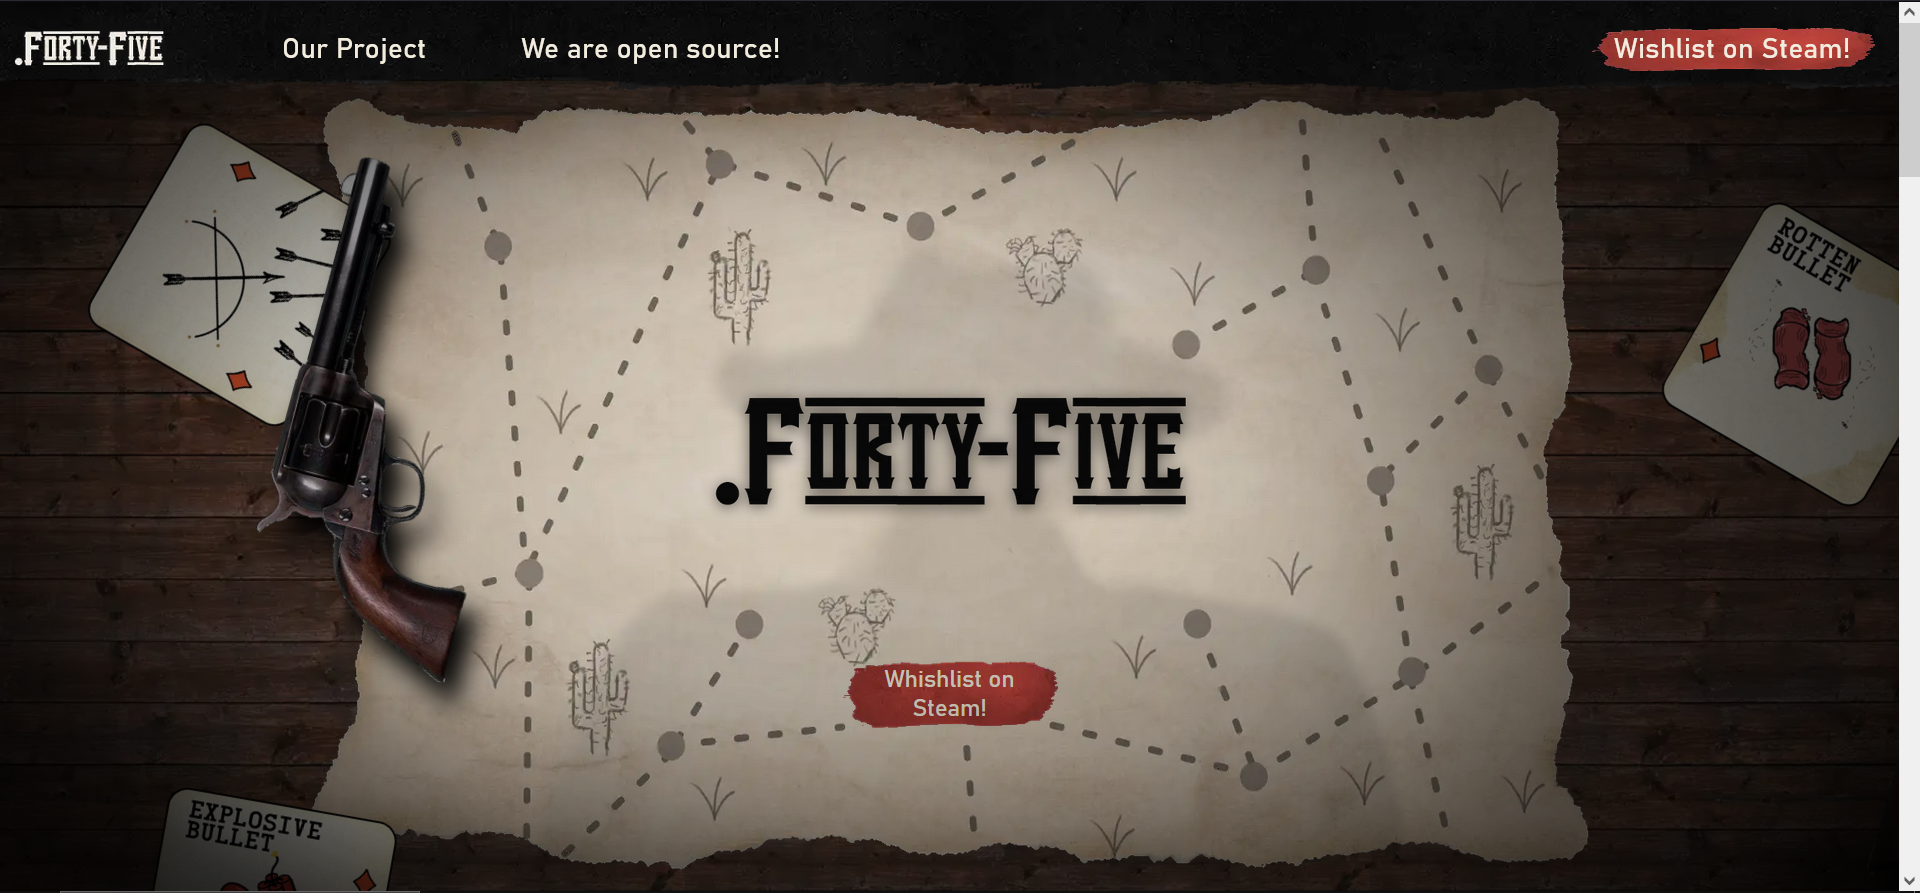
\includegraphics[width=1.0\textwidth]{website.png}
    \caption{Screenshot der Website}
\end{figure}

Das wirkt sich natürlich negativ auf die Ladezeiten der Website aus.
Um diesen Effekt so gering wie möglich zu halten, wurde das von Google entwickelte webp Bild-Format verwendet, welches
eine deutlich bessere Komprimierung als vergleichbare Formate wie \zB jpg erzielt.
In einer vergleichenden Studie, welche von Google durchgeführt wurde, erreichte webp je nach verwendeter Methodik eine
Verkleinerung von 14\% gegenüber eines mit jpg komprimierten Bildes.\zit{googleWebpStudie}

% resets author
\renewcommand{\kapitelautor}{}
